%
% points.tex
%
\section{Chart::Points}
\name{Chart::Points}
\file{Points.pm}
\requires{Chart::Base, GD, Carp, FileHandle}
\begin{Description} 
\class{Points} is a subclass of class \class{Chart::Base}.\\
The class Points creates a point chart.
\end{Description}

\parindent 0pt{\large Example:}

\begin{figure}[h]
	\begin{center}
		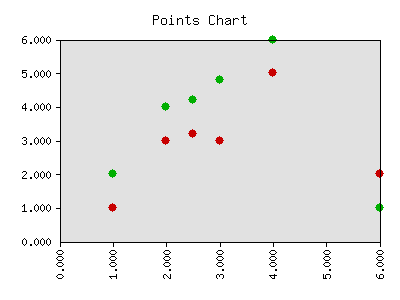
\includegraphics[scale=0.5]{points.png}
	\end{center}
	\caption{Points chart}
	\label{fig:points}
\end{figure}
\begin{verbatim}
use Chart::Points;

$g = Chart::Points->new();
$g->add_dataset (1, 4,   3, 6, 2, 2.5);  # x-coordinates
$g->add_dataset (1, 5,   3, 2, 3, 3.2);  # y-coordinates dataset 1
$g->add_dataset (2, 6, 4.8, 1, 4, 4.2);  # y-coordinates dataset 2

@hash = ('title' => 'Points Chart',
         'xy_plot' => 'true',
         'x_ticks' => 'vertical',
         'legend' => 'none',
         'sort' => 'true',
         'precision' => 3,
         'include_zero' => 'true',
	 );

$g->set (@hash);

$g->png ("Grafiken/points.png");
\end{verbatim}

\begin{Constructor} 
An instance of a points chart object can be created with the constructor \textit{new()}:
\begin{quote}
\fett{\$obj = Chart::Points->new();}\\
\fett{\$obj = Chart::Points->new(\parameter{width}, \parameter{height});}
\end{quote}

If \textit{new()} has no arguments, 
the constructor returns an image with the size 300x400 pixels. If new has two arguments 
\parameter{width} and \parameter{height}, 
it returns an image with the desired size.
\end{Constructor}

\Methods
All universal valid methods, see page \pageref{methods} of class \class{Chart::Base}. \\[\parabstand]
%
\Attributes
All universal valid options, see page \pageref{options}. 
Also available these special options:
\begin{description}
\item['y\_axes'] Tells chart where to place the y-axis. 
                 Valid values are 'left', 'right' and 'both'. Defaults to 'left'.
                 
\item['pt\_size'] Sets the radius of the points in pixels. Default is 18.

\item['sort'] Sorts the data of a x-y-graph ascending if set to 'true'. 
              Should be set if the added data isn't sorted. Defaults to 'false'.
              
\item['xy\_plot'] Forces Chart to plot a x-y-graph, 
                  which means that the x-axis is also numeric if set to 'true'. 
                   Very useful for plots of mathematical functions. Defaults to 'false'.

\item['xlabels', 'xrange'] Allows the arbitrary positioning of the labels at the
                  x-axis. The option 'xy\_plot' must be defined to let this
                  options work. An example is
                  \begin{verbatim}
@labels = (['Jan', 'Feb','Mar'], 
           ['10','40','70']); 

$chart->set( xlabels => \@labels, 
             xrange => [0,100] 
           ); 
                   \end{verbatim}

\end{description}
